% !TEX TS-program = XeLaTeX
% use the following command: 
% all document files must be coded in UTF-8
\documentclass{textolivre}
% See more information on the repository: https://github.com/leolca/textolivre

% Metadata
\begin{filecontents*}[overwrite]{article.xmpdata}
    \Title{Jogos digitais e acentuação gráfica: conexões possíveis entre aprendizagem e ludicidade}
    \Author{Ana Luiza de Souza Couto \sep Letícia Pena Silveira \sep Marcelo de Castro}
    \Language{pt-BR}
    \Keywords{Jogos digitais \sep Ensino-aprendizagem \sep Ludicidade \sep Acentuação gráfica}
    \Journaltitle{Texto Livre}
    \Journalnumber{1983-3652}
    \Volume{14}
    \Issue{3}
    \Firstpage{1}
    \Lastpage{17}
    \Doi{10.35699/1983-3652.2021.35333}

    \setRGBcolorprofile{sRGB_IEC61966-2-1_black_scaled.icc}
            {sRGB_IEC61966-2-1_black_scaled}
            {sRGB IEC61966 v2.1 with black scaling}
            {http://www.color.org}
\end{filecontents*}

\journalname{Texto Livre}
\thevolume{14}
\thenumber{3}
\theyear{2021}
\receiveddate{\DTMdisplaydate{2021}{7}{21}{-1}} % YYYY MM DD
\accepteddate{\DTMdisplaydate{2021}{9}{2}{-1}}
\publisheddate{\DTMdisplaydate{2021}{9}{15}{-1}}
% Corresponding author
\corrauthor{Marcelo de Castro}
% DOI
\articledoi{10.35699/1983-3652.2021.35333}
%\articleid{NNNN} % if the article ID is not the last 5 numbers of its DOI, provide it using \articleid{} commmand
% Abbreviated author list for the running footer
\runningauthor{Couto et al.}
\sectioneditorname{Daniervelin Pereira}
\layouteditorname{Anna Izabella M. Pereira}


\title{Jogos digitais e acentuação gráfica: conexões possíveis entre aprendizagem e ludicidade}
\othertitle{Digital games and accent mark: possible connections between learning and playfulness}
% if there is a third language title, add here:
%\othertitle{Artikelvorlage zur Einreichung beim Texto Livre Journal}

\author[1]{Ana Luiza de Souza Couto~\orcid{0000-0002-6389-7818} \thanks{Email: \url{annaluizasouzacouto@hotmail.com}}}
\author[1]{Letícia Pena Silveira~\orcid{0000-0003-1194-3437} \thanks{Email: \url{leticiapenasilveira@hotmail.com}}}
\author[1]{Marcelo de Castro~\orcid{0000-0002-1056-1288} \thanks{Email: \url{marcelocastromc@hotmail.com}}}

\affil[1]{Universidade Federal de Minas Gerais, Faculdade de Letras, Belo Horizonte, MG, Brasil.}

\addbibresource{article.bib}
% use biber instead of bibtex
% $ biber tl-article-template

% set language of the article
\setdefaultlanguage{portuguese}
\setotherlanguage{english}

% for spanish, use:
%\setdefaultlanguage{spanish}
%\gappto\captionsspanish{\renewcommand{\tablename}{Tabla}} % use 'Tabla' instead of 'Cuadro'
%\AfterEndPreamble{\crefname{table}{tabla}{tablas}\Crefname{table}{Tabla}{Tablas}}

% for languages that use special fonts, you must provide the typeface that will be used
% \setotherlanguage{arabic}
% \newfontfamily\arabicfont[Script=Arabic]{Amiri}
% \newfontfamily\arabicfontsf[Script=Arabic]{Amiri}
% \newfontfamily\arabicfonttt[Script=Arabic]{Amiri}
%
% in the article, to add arabic text use: \textlang{arabic}{ ... }

% for russian text we also need to define fonts with support for Cyrillic script
% \usepackage{fontspec}
% \setotherlanguage{russian}
% \newfontfamily\cyrillicfont{Times New Roman}
% \newfontfamily\cyrillicfontsf{Times New Roman}[Script=Cyrillic]
% \newfontfamily\cyrillicfonttt{Times New Roman}[Script=Cyrillic]
%
% in the text use \begin{russian} ... \end{russian}

% to use emoticons in your manuscript
% https://stackoverflow.com/questions/190145/how-to-insert-emoticons-in-latex/57076064
% using font Symbola, which has full support
% the font may be downloaded at:
% https://dn-works.com/ufas/
% add to preamble:
% \newfontfamily\Symbola{Symbola}
% in the text use:
% {\Symbola }

% reference itens in a descriptive list using their labels instead of numbers
% insert the code below in the preambule:
\makeatletter
\let\orgdescriptionlabel\descriptionlabel
\renewcommand*{\descriptionlabel}[1]{%
  \let\orglabel\label
  \let\label\@gobble
  \phantomsection
  \edef\@currentlabel{#1\unskip}%
  \let\label\orglabel
  \orgdescriptionlabel{#1}%
}
\makeatother
%
% in your document, use as illustraded here:
%\begin{description}
%  \item[first\label{itm1}] this is only an example;
%  % ...  add more items
%\end{description}
 

% custom epigraph - BEGIN 
%%% https://tex.stackexchange.com/questions/193178/specific-epigraph-style
\usepackage{epigraph}
\renewcommand\textflush{flushright}
\makeatletter
\newlength\epitextskip
\pretocmd{\@epitext}{\em}{}{}
\apptocmd{\@epitext}{\em}{}{}
\patchcmd{\epigraph}{\@epitext{#1}\\}{\@epitext{#1}\\[\epitextskip]}{}{}
\makeatother
\setlength\epigraphrule{0pt}
\setlength\epitextskip{0.5ex}
\setlength\epigraphwidth{.7\textwidth}
% custom epigraph - END


% if you use multirows in a table, include the multirow package
\usepackage{multirow}

% add line numbers for submission
%\usepackage{lineno}
%\linenumbers

\begin{document}
\maketitle

\begin{polyabstract}
\begin{abstract}
Embora os jogos digitais sejam vistos de forma pejorativa por pais e professores \cite{leffa2012}, eles são objetos de ensino-aprendizagem que podem beneficiar a leitura e a escrita \cite{ribeiro2016}. No que se refere à acentuação, não é raro escutar colocações, por parte de alguns docentes, sobre a ausência e/ou o uso errado de acento gráfico nos textos formais escritos pelos alunos \cite{couto+guimaraes2020}. Nesse contexto, este estudo articula a acentuação gráfica – que se apresenta como um conteúdo de difícil ensino – e os jogos – ferramentas capazes de contribuir para uma prazerosa aprendizagem. Assim, o objetivo foi analisar jogos digitais voltados à aprendizagem da acentuação gráfica, de modo a discutir as conexões possíveis entre aprendizagem e ludicidade inerentes (ou não) a eles. Este trabalho pauta-se nas teorizações sobre os jogos digitais \cite{leffa2012, ribeiro2013, ribeiro2016} e o ensino-aprendizagem da acentuação gráfica \cite{marra2012, couto+guimaraes2020, cristofaro2020}. Metodologicamente, trata-se de uma investigação descritivo-interpretativista de abordagem qualitativa \cite{paiva2019}. Os resultados evidenciaram que os jogos analisados foram construídos sob a égide do ensino mecânico e descontextualizado da escrita, com foco na memorização, e propiciam uma aprendizagem tímida com ludicidade mínima ou nula.

\keywords{Jogos digitais \sep Ensino-aprendizagem \sep Ludicidade \sep Acentuação gráfica}
\end{abstract}

\begin{english}
\begin{abstract}
Although digital games have been seeing in a pejorative way by parents and teachers \cite{leffa2012}, they are teaching-learning objects that can benefit reading and writing \cite{ribeiro2016}. With regard to accent mark, it is common to hear some teachers statements about the absence and/or wrong use of accent mark in formal texts written by students \cite{couto+guimaraes2020}. Considering this context, this paper articulates accent mark – which presents itself as a difficult teaching content – and games – tools capable of contributing to a pleasurable learning experience. Thus, the objective was to analyze digital games in accent mark learning, in order to discuss the possible connections between learning and playfulness inherent (or not) to them. This work is based on theories about digital games \cite{leffa2012, ribeiro2013, ribeiro2016} and the teaching-learning of accent mark \cite{marra2012, couto+guimaraes2020, cristofaro2020}. Methodologically, it is a descriptive-interpretative investigation with a qualitative approach \cite{paiva2019}. The results showed that the analyzed games were built under the aegis of mechanical teaching and decontextualized writing, with a focus on memorization, and provide a timid learning with minimal or no playfulness.

\keywords{Digital games \sep Teaching-learning \sep Playfulness \sep Accent mark}
\end{abstract}
\end{english}

% if there is another abstract, insert it here using the same scheme
\end{polyabstract}


\section{Introdução}\label{sec-intro}
Embora, muitas vezes, sejam vistos de forma pejorativa por pais e professores \cite{leffa2012}, os jogos digitais são objetos de ensino-aprendizagem que podem beneficiar a leitura e a escrita \cite{ribeiro2016}, ou seja, que podem ser potenciais fontes para aprendizagem de línguas \cite{leffa2012}. Muitas investigações já foram desenvolvidas a respeito da existência (assim como da pertinência) de jogos digitais no contexto da alfabetização \cite{coscarelli2013, ribeiro2012, ribeiro2013, ribeiro2009}. De modo geral, elas explicitam o poder de tais recursos tecnológicos para produção de conhecimento sobre nosso sistema alfabético. Porém, a maioria desses estudos trouxe evidências de que a ludicidade – despertadora e motivadora do interesse de um jogador – não está muito presente nos games, o que se opõe a um pressuposto básico de que o entretenimento é, sim, uma qualidade para se conceituar um bom jogo \cite{leffa2012}.

Contudo, quando são analisados jogos digitais – direcionados a um público infanto-juvenil e/ou adulto, isto é, a sujeitos teoricamente que já dominam o código alfabético e estão em uma etapa de escolarização mais avançada – essa situação (em que aprendizagem e ludicidade não se associam plenamente) se mantém em tais ferramentas? A partir dessa pergunta norteadora ampla, objetiva-se, neste artigo, analisar jogos digitais voltados à aprendizagem da língua portuguesa, especificamente a acentuação gráfica, de modo a discutir as conexões possíveis entre aprendizagem e ludicidade inerentes (ou não) a eles. Para tanto, foram selecionados dois jogos digitais que tematizam a acentuação gráfica e que podem ser acessados e/ou baixados gratuitamente pelo usuário: Bruxa dos Acentos\footnote{Disponível em: \url{http://www.escolagames.com.br/jogos/bruxaDosAcentos/}.} e Acentuando\footnote{Disponível em: {\url{https://play.google.com/store/apps/details?id=br.estacio.ead.AcerteAcento&hl=pt_BR&gl=US}.}}. A análise dos jogos está embasada em 10 critérios: 7 didático-pedagógicos – 1) Concepção de língua, 2) Tipos de ensino, 3) Disposição do objetivo e do conteúdo, 4) Recursos e Interatividade, 5) Motivação, 6) \emph{Feedback}, 7) Sistemas de ajuda; e 3 ergonômicos: 1) Usabilidade, 2) Acessibilidade, 3) Funcionalidade – que serão detalhados adiante com embasamento em \textcite{ribeiro2009} e em \textcite{ribeiro2013}, assim como nas teorizações sobre jogos digitais \cite{gee2004, leffa2012, ribeiro2016} e a acentuação gráfica \cite{brasil2008, collischonn2005, marra2012, cristofaro2020, couto+guimaraes2020}. Metodologicamente, trata-se, portanto, de um estudo de abordagem qualitativa \cite{paiva2019} cujo alvo é a descrição e a interpretação subjetiva de jogos digitais sobre a acentuação gráfica – componente da ortografia que, ainda, possui desafios em relação ao seu ensino-aprendizagem nas aulas de língua portuguesa \cite{couto+guimaraes2020}.

Justifica-se o interesse pelos jogos digitais ao se considerar que, a cada dia mais, as tecnologias digitais fazem parte da sociedade, e a escola não pode ignorar tal questão, uma vez que os alunos, comumente, estão imersos nesse universo. Como aponta \textcite{coscarelli2016}, as tecnologias supracitadas devem ser amplamente pesquisadas, debatidas e empregadas nas instituições de ensino. \textcite{gee2004} também argumenta a favor da relevância dos jogos – não só em ambientes educativos, mas na vida em geral de qualquer indivíduo – e da seriedade desses recursos no que se refere à aprendizagem, sem perder de vista a diversão. Acredita-se que os jogos digitais podem ser proveitosos para o desenvolvimento dos aspectos linguísticos, sociais e cognitivos dos discentes, do interesse pela disciplina e do pensamento criativo, uma vez que trariam à aprendizagem mais dinamicidade e interação.

No que se refere à acentuação gráfica, conteúdo recortado para a presente discussão – não é raro escutar colocações, por parte de alguns docentes, sobre a ausência e/ou o uso errado de acento gráfico (agudo, circunflexo e/ou grave) nos textos formais escritos pelos estudantes \cite{cristofaro2020, couto+guimaraes2020}. Esse discurso, de acordo com \textcite{couto+guimaraes2020}, também pode ser verbalizado pelos próprios discentes que, para além das sinalizações em suas produções textuais, explicitam desconhecimento ou dúvidas quanto à acentuação gráfica. Ainda que as pessoas possam contar com corretores ortográficos em programas digitais, presentes em computadores e celulares, a ortografia é um saber que não pode ser negligenciado, pois escritores que despendem demasiada atenção a ela acabam por ter mais dificuldades para se dedicarem a outros aspectos inerentes à escrita \cite{treiman2014}. Além do mais, conforme a Base Nacional Comum Curricular – BNCC \cite{brasil2017, brasil2018}, tanto alunos do Ensino Fundamental II quanto do Médio precisam demonstrar habilidade no uso de conhecimentos de aspectos notacionais, como a ortografia, nas práticas de escrita. O domínio da escrita ortográfica, enquanto uma das facetas da língua, contribui para a formação do sujeito letrado capaz de utilizar a escrita nos mais diversos contextos sociais \cite{soares2004, soares2018}. Então, a acentuação é um conhecimento linguístico tido como um direito de aprendizagem a ser assegurado pelas aulas de língua portuguesa \cite{brasil2018}. Nesse contexto, este estudo concilia dois pontos essenciais: a acentuação gráfica – que se apresenta como um conteúdo de difícil ensino e aprendizagem na educação básica – e os jogos digitais – ferramentas capazes de contribuir para a aprendizagem dos alunos, em específico, a respeito da acentuação.

Quanto à organização do artigo, além desta primeira seção (\ref{sec-intro}), Introdução, em que foi, sumariamente, construído um “desenho” investigativo, há mais seis seções. Na segunda (\ref{sec-2}), é feita uma caracterização dos jogos digitais e uma problematização sobre o uso deles no processo de ensino-aprendizagem. Na terceira (\ref{sec-3}), a acentuação gráfica é localizada como um componente da escrita ortográfica, assim como é pensada a partir da concepção de língua que se adota. Na quarta (\ref{sec-4}), são apresentados os procedimentos metodológicos adotados para realização da pesquisa, para, em seguida, na quinta (\ref{sec-5}), os jogos serem descritos e analisados. Na sexta (\ref{sec-6}), tendo em vista os resultados alcançados e os fundamentos teóricos, são construídas proposições de como aprendizagem e ludicidade podem ser articuladas na criação e/ou na atualização de futuros jogos digitais sobre acentuação. Por fim, na última seção (\ref{sec-7}), são engendradas as considerações finais.

\section{Jogos digitais no ensino-aprendizagem de língua}\label{sec-2}
De acordo com \textcite{gee2004}, os jogos são fenômenos culturais que fazem parte da vida das pessoas desde a mais tenra idade. Os jogos digitais, especificamente, estão em meio eletrônico e podem ser definidos, nas palavras de \textcite[p. 7]{schuytema2016}, como “uma atividade lúdica composta por uma série de ações e decisões, limitado por regras e pelo universo do game, que resultam em uma condição final”. Para \textcite{gee2004}, tais jogos podem pertencer a diferentes gêneros, como de tiro, de estratégia, de simulação, RPG (\emph{Role Playing Game}), entre outros.

Segundo \textcite[p. 13]{coscarelli2016}, “os jogos desenvolvem memória, criatividade, raciocínio, solução de problemas, bem como ajudam os jogadores a lidar com a frustração e a trabalhar colaborativamente”. Por tudo isso, já está mais que reconhecido o quanto os jogos digitais oportunizam, sim, aprendizagens \cite{gee2004, jones2004, ribeiro2016}. Inclusive, é pela via da aprendizagem e do desafio que os jogos se tornam divertidos e motivadores para os sujeitos \cite{gee2009}.

\textcite[p. 218]{leffa2012}, por sua vez, ao discutirem o potencial didático do videogame na aprendizagem de línguas, afirmam que este “é um gênero do discurso multimodal que se define pela presença de determinadas características como ludicidade, interatividade, imprevisibilidade, suporte eletrônico, ação física do jogador”. Algumas dessas características, em especial as três primeiramente citadas, podem aparecer em maior ou menor escala, isto é, a interatividade com o jogador pode ser contínua ou acontecer em raros momentos do game, por exemplo. As outras categorias, como suporte eletrônico e ação física do jogador, não são medidas em uma gradação (como as anteriores), mas se dão de modo terminante, ou seja, sempre haverá um suporte eletrônico e serão necessárias ações do jogador para que o jogo seja executado \cite{leffa2012}.

Ao se pensar na qualidade de um jogo, \textcite{leffa2012} definem que um bom jogo é aquele que vicia, isto é, que preza mais pelo entretenimento do que, necessariamente, pela aprendizagem. Por essa razão, “um jogo pedagógico com ênfase no uso de recursos interativos, mas com baixo valor de entretenimento, ficaria na fronteira entre o videogame e o exercício didático” \cite[p. 219]{leffa2012}. Logo, ao se considerar o processo de ensino-aprendizagem, um jogo digital pode ser bem avaliado quando agrega aprendizagem e ludicidade.

Além de favorecer a aprendizagem de conteúdos específicos, como a respeito da escrita ortográfica do português brasileiro (doravante PB), um jogo digital, por ser multimodal, ou seja, por associar diferentes linguagens, também requer “que o jogador entenda as regras do jogo e descubra como operá-las por meio do manuseio de botões, janelas, abas, ícones, links etc.” \cite[p. 166]{ribeiro2016}. Isso significa que, por meio de um game – em que diversos elementos multimodais, gráficos e de navegação precisam ser identificados, interpretados e bem usados pelo jogador –, também é possível promover o letramento digital, conceito que recobre as práticas sociais de leitura e de escrita em ambientes digitais \cite{ribeiro2014}. Por mais que a leitura do texto digital não seja uma ruptura com aquela feita a partir do impresso \cite{ribeiro2008}, não se pode negar que há algumas habilidades demandadas em um jogo digital, como as citadas, que são diferentes de outras exigidas no papel.

Desse modo, a ideia – bastante recorrente no imaginário social – de que jogos são perda de tempo é uma grande falácia, pois algo sempre pode ser aprendido com eles \cite{gee2004}. Nesse sentido, \textcite{gee2004} afirma que, mesmo quando não há um conteúdo escolar explícito, lidar com um novo domínio semiótico, como acontece ao jogar um videogame, abarca, por exemplo, aprender a experienciar o mundo (em diferentes e novos modos de sentir, ver, operar) e obter recursos preparatórios para aprendizados a posteriori.

Quanto à aplicação de tecnologias digitais (como jogos) no ensino, corrobora-se o dizer de \textcite{ribeiro2020} de que isso acontece de forma tímida. De acordo com \textcite{ribeiro2016}, depois dos primeiros anos do Ensino Fundamental, não é comum haver o emprego de jogos no processo de ensino da língua portuguesa. Para a autora, dois fatos podem justificar essa ausência: o primeiro refere-se à concepção de parte dos professores de que jogos são recursos meramente voltados à ludicidade, isto é, sem um potencial para explorar conteúdos escolares; o segundo diz respeito à falta de conhecimento de muitos profissionais dos anos finais do Ensino Fundamental e do Ensino Médio a respeito da forma como os jogos podem fazer parte da prática pedagógica.

Nessa lógica, devido a crenças equivocadas, a formações docentes deficitárias na questão e, até mesmo, à pouca oferta de jogos digitais, verifica-se que estes, geralmente, não são usados no ensino de língua materna como mais uma ferramenta que colabora para o aprimoramento das habilidades letradas. Em contrapartida, cada vez mais, crianças e adultos estão interessados em jogos digitais, e a indústria, nesse ramo, cresce exponencialmente \cite{ribeiro2016}. Diante desse cenário no qual se vê um abismo entre as práticas sociais fora e dentro dos muros escolares, urge analisar jogos digitais sobre a língua portuguesa, principalmente quanto à aprendizagem e à ludicidade, a fim de se (re)pensar em alternativas à problemática. Antes de se chegar a essa etapa, cabe esclarecer algumas noções sobre o conteúdo dos jogos digitais escolhidos: a acentuação gráfica.

\section{Acentuação: especificidades linguísticas e concepções de língua}\label{sec-3}
A ortografia do PB é regida por regras, que entraram em vigor, no Brasil, pela legislação do novo Acordo Ortográfico em 2008 \cite{brasil2008}. Além de definir quais grafemas são utilizados para grafar as palavras, o Acordo Ortográfico também assegura o uso de diacríticos, tais como o til (ã), o pingo no <i>, o acento grave (à), o acento agudo (á) e o acento circunflexo (â), além das mais diversas pontuações. Nesse sentido, o acento gráfico, foco deste artigo, atua como um componente da ortografia do PB. O conhecimento e o domínio de tais regras contribui para a construção de um estudante letrado capaz de fazer o uso das facetas da língua nos mais diversos contextos sociais \cite{soares2004, soares2018}. Para desenvolver a análise dos jogos digitais, é preciso, antes de tudo, contextualizar o que é o acento tônico, seus aspectos fonéticos e fonológicos, para, posteriormente, relacioná-lo ao acento gráfico.

O acento tônico é inerente à língua e refere-se “à proeminência de uma vogal em relação às demais vogais do enunciado”, mas que, comumente, é referido à sílaba \cite[p. 44]{cristofaro2017}. Suas características fonéticas são definidas de acordo com a intensidade, a altura e a duração da vogal \cite{cantoni2013, cristofaro2017}. Muitos estudos foram desenvolvidos em relação ao acento no PB a partir de um viés fonológico \cite{collischonn2005, cantoni2013}. Como referido por \textcite{camara1970}, o acento possui duas funções importantes no PB, a delimitativa e a distintiva. A primeira refere-se à delimitação de palavras no curso sonoro da fala; por exemplo, devido ao acento, o falante consegue distinguir  “mesa das bebidas” e “mesadas bebidas” \cite[p. 17]{ferreira2007}. Já a segunda função, a distintiva, refere-se à distinção de palavras que possuem a mesma cadeia sonora, como em “\textbf{sá}bia [ˈsa.bi.a], sa\textbf{bi}a [sa.ˈbi.a] e sabiá [sa.bi.ˈa]” \cite{camara1970}.

Além disso, há regras gerais em relação ao acento tônico, que fazem parte da gramática do PB, tais como: ele ocorre apenas nas três últimas sílabas e pode ser classificado como proparoxítono, quando o acento recai na antepenúltima sílaba (\textbf{mé}dico, fo\textbf{né}tica), paroxítono, quando a sílaba tônica é a penúltima (\textbf{ál}bum, a\textbf{mi}go), e oxítono, quando o acento marca a vogal da última sílaba (ca\textbf{fé}, uru\textbf{bu}). Ademais, no PB, o acento tem preferência pela posição paroxítona, a vogal da penúltima sílaba \cite{collischonn2005}. Ou seja, a frequência de palavras com o acento tônico na posição paroxítona é maior em relação às posições proparoxítona e oxítona, como em “mesa”, “roupa”, “amigo”, “vizinho”, “proibido”, entre outras. Por isso, há mais palavras paroxítonas que não recebem a acentuação gráfica, exceto alguns casos\footnote{Há palavras paroxítonas que são acentuadas graficamente, como amável, ágil, órfão, entre outras.}, do que o contrário, visto que o acento tônico paroxítono já é marcado na língua portuguesa, e não necessita da marcação gráfica \cite{cantoni2013}.

Até aqui, discorreu-se sobre o acento tônico e se notou que há regras linguísticas relacionadas a este acento que fazem parte da gramática do PB. O acento tônico e o acento gráfico compartilham algumas características, no entanto, é importante distingui-los. O primeiro é inerente à língua, e todas as palavras, exceto os monossílabos átonos, recebem o acento tônico. Já o segundo diz respeito a “parâmetros específicos que visam à economia, não-redundância” \cite[p. 140]{couto+guimaraes2020}, sendo ele representado, na escrita, pelo acento agudo (´) – nas vogais tônicas abertas – e o circunflexo (\^) – nas vogais tônicas fechadas, além disso, ele é regido por regras estabelecidas pelo novo Acordo Ortográfico \cite{brasil2008}. O acento tônico nem sempre é marcado pelo acento gráfico, como em du\textbf{vi}da [du.ˈvi.də], mas também os dois podem se acumular na mesma vogal, como em \textbf{dú}vida [ˈdu.vi.də]. O acento gráfico, portanto, “permite ao leitor distinguir como pronunciar uma palavra da maneira adequada” \cite[p. 437]{cristofaro2020}. Assim como o acento tônico, o gráfico ocorre apenas em três posições na palavra, proparoxítona, paroxítona e oxítona. Todas as regras da acentuação gráfica estão dispostas no novo Acordo Ortográfico \cite{brasil2008}, além de diversos trabalhos de linguistas e gramáticos, como \textcite{rochalima2011, marra2012, luft2013} etc.

De acordo com as regras da acentuação gráfica, o acento gráfico exige diferentes conhecimentos linguísticos para o seu entendimento, como os sons abertos, as vogais abertas – que recebem o acento agudo – (como avó), e os sons fechados, vogais fechadas – que recebem o acento circunflexo – (como em avô); a posição da vogal tônica na palavra, se é antepenúltima, penúltima e última. Ademais, é importante o conhecimento das funções da palavra em contexto específico, como verbos, nomes, adjetivos, para a compreensão de como o acento tônico e o gráfico podem modificar a classe da palavra, como \textbf{dú}vida e du\textbf{vi}da; bo\textbf{tão} e \textbf{bo}tam; \textbf{es}ta e es\textbf{tá}, sobretudo, na diferença entre acento tônico e gráfico. Nesse ínterim, é importante que o ensino do acento gráfico seja de acordo com a faixa etária do aprendiz, consoante os aspectos linguísticos que estão sendo desenvolvidos em cada segmento escolar. Também é de suma importância que o ensino da acentuação gráfica seja reflexivo e seja realizado a partir da realidade dos discentes, com palavras que são frequentes para eles \cite{couto+guimaraes2020}.

Além dos diacríticos relacionados à acentuação gráfica – circunflexo e agudo – na ortografia do português brasileiro, também há o acento grave, que indica a marcação da “crase: \emph{à} ou \emph{àquela}” \cite[p. 130]{cristofaro2017}. A crase refere-se à fusão de dois ‘a’, a preposição mais o artigo, e é regulada por diversas regras gramaticais. Tendo em vista seu caráter multifacetado, a compreensão do seu uso envolve conhecimentos sintáticos e semânticos, como o contexto de verbos e demais palavras.

Infelizmente, o domínio da acentuação gráfica ainda enfrenta desafios nos mais diversos segmentos educacionais brasileiros, como no Ensino Fundamental I \cite{marra2012, ney2019, cristofaro2020}, no Fundamental II \cite{couto+guimaraes2020}, no Médio \cite{sartori2015} e até mesmo no Superior em Portugal \cite{castelo2017}. Soma-se a essa defasagem a escassez de direcionamentos do ensino reflexivo do acento gráfico em documentos educacionais brasileiros, como a BNCC \cite{brasil2017, brasil2018}, e em livros didáticos (adotados nas escolas brasileiras), nos quais são propostas atividades pautadas na memorização de regras, que não propiciam ao aluno reflexões sistematizadas sobre os aspectos da acentuação gráfica \cite{couto2020}. Diante disso, o jogo digital – de forma lúdica, mais atrativa e interessante – poderia contribuir para a resolução dessa problemática que envolve o ensino e a aprendizagem do acento gráfico na educação brasileira.

Contudo, lamentavelmente, o ensino do acento gráfico nas escolas ainda é pautado na exposição e na memorização de regras. Isso advém de diversas concepções de língua presentes nas salas de aula de LP, as quais afirmam que a aprendizagem da escrita ortográfica ocorre, apenas, por meio da memorização de regras, e não por meio da reflexão de aspectos linguísticos do PB \cite{costa_val1996, couto2020}. Sendo a acentuação gráfica um componente da ortografia, ela também é afetada por diversas concepções de língua, que, comumente, perpassam os caminhos do discente da educação básica brasileira durante o processo de aprendizagem da escrita ortográfica. Portanto, o ensino-aprendizagem da acentuação gráfica, por meio dos jogos digitais, pode, também, ser estruturado por diferentes concepções de língua1 que precisam ser discutidas para a avaliação dos jogos. Sendo assim, a seguir, serão tecidas discussões sumárias sobre três concepções de língua que estão presentes no ensino da LP: Estruturalismo, Gerativismo e Sociointeracionismo.

Ancorada nos estudos do linguista \textcite{saussure2006} – pai da linguística moderna –, há a corrente estruturalista, na qual a concepção de língua é pautada na estrutura, tida como um código concreto e, assim, não se consideram as diversas formas de realização na fala. Nessa perspectiva, a língua, inclusive a escrita, é apenas aprendida por meio da memorização, sobretudo, das regras que compõem a língua padrão \cite{costa_val1996, couto2020}. Além disso, as atividades que envolvem a ortografia, na perspectiva estruturalista, são pautadas em preenchimento de lacunas, memorização de palavras, sem haver a reflexão das facetas da língua.

Com a evolução dos estudos linguísticos, surgiu a corrente do Gerativismo, pautada nos estudos de \textcite{chomsky1986}. O gerativismo assume a língua como capacidade inata de qualquer indivíduo, constituída por regras universais, e vista como um reflexo da atividade mental, em outras palavras, a língua como expressão do pensamento \cite{costa_val1996, couto2020}. Nessa lógica, o ensino da língua escrita é pautado na memorização de regras, como um reflexo da mente, e não há espaço para as reflexões das diversas realizações da língua, tanto na fala, quanto na escrita. Há, também, no gerativismo, a descrição de regras, atividades com palavras isoladas, mas sem a reflexão e o contexto de uso de tais regras.

Como uma nova proposta, há a concepção de língua como interação, ancorada em \textcite{bakhtin2006}, denominada sociointeracionista. Essa concepção (defendida neste artigo) vai de encontro ao Estruturalismo e ao Gerativismo, pois considera a língua como meio de interação entre os falantes dentro de um contexto social \cite{couto2020}. Sendo assim, o ensino da escrita ortográfica é pautado na reflexão dos aspectos ortográficos dentro de um contexto de uso, além disso, não é mais necessária a memorização, pois o discente é instigado a investigar e refletir sobre o uso das normas ortográficas. No quesito do ensino da acentuação gráfica, essa perspectiva, atrelada aos jogos digitais educacionais, poderá contribuir para a formação do aluno letrado, capaz de utilizar as facetas da língua, fala e escrita, nos mais diversos contextos sociais \cite{soares2004}. Compreendidos os aspectos teóricos, na seção a seguir, é apresentada a metodologia utilizada no desenvolvimento deste trabalho.

\section{Metodologia}\label{sec-4}
Este estudo configura-se como uma investigação descritivo-interpretativista de abordagem qualitativa \cite{paiva2019}. Isso porque se tem como objetivo descrever e analisar um fenômeno social, neste caso, o ensino da acentuação gráfica em jogos ou atividades digitais voltados para o ensino-aprendizagem de língua portuguesa. Para a realização da pesquisa, foram seguidas as seguintes etapas:

- Etapa I: Levantamento dos jogos educativos destinados ao ensino de língua portuguesa para alunos a partir das séries finais do Ensino Fundamental I. Nessa busca, foram encontrados muitos exemplos voltados ao ensino do referido componente curricular, porém poucos tinham exclusividade na questão da acentuação gráfica. Diante disso, para a seleção dos objetos de análise, foram estipulados os seguintes critérios:

\begin{enumerate}[label=\alph*]
    \item Ser de acesso gratuito;
    \item Ter classificação de conteúdo com faixa etária livre ou a partir de 07 anos;
    \item Estar disponível para acesso durante a escrita deste artigo;
    \item Permitir o uso por um ou mais jogadores;
    \item Ter foco no conteúdo da acentuação gráfica; 
    \item Ser nomeado pelo fabricante como jogo.
\end{enumerate}

A partir disso, para o corpus desta pesquisa, selecionou-se um jogo colhido de \emph{website} e uma atividade digital disponível na loja de aplicativos para celulares. São eles:

\begin{itemize}
    \item Bruxa dos Acentos, criado pela Escola Game.
    \item Acentuando, produzido pela Estácio de Sá. Recebeu a última atualização em abril de 2016.
\end{itemize} 

- Etapa II: Seleção dos critérios que foram utilizados para a análise do nível de aprendizado e de ludicidade. Para tanto, recorreu-se a dois trabalhos, o de \textcite{ribeiro2009} e o de \textcite{ribeiro2013}, a fim de verificar aqueles utilizados pelas autoras e, a partir disso, elaborar os dez que foram usados neste artigo. Estes foram divididos em dois âmbitos para melhor avaliação: o didático-pedagógico (7) e o ergonômico (3). Em relação aos critérios didático-pedagógicos, tem-se:

\begin{enumerate}
    \item \textbf{Concepção de língua:} para \textcite{ribeiro2013}, o ideal é que os jogos sejam pautados na perspectiva da língua como interação, já que, assim, “os fenômenos da língua seriam trabalhados em função dos textos (reais, concretos)” \cite[p. 73-74]{ribeiro2013}. \textcite{ribeiro2009} seguem a mesma linha ao afirmarem que os jogos devem estimular a aprendizagem ativa, construtiva e contextualizada. 
    \item \textbf{Tipo de ensino:} \textcite{ribeiro2013} refere-se aos tipos prescritivo, que leva em consideração a memorização das regras; ao descritivo, o qual é baseado na descrição do funcionamento da língua e, portanto, na repetição dos exercícios; e o tipo produtivo, que permite ao aluno entender as relações linguísticas com um ensino contextualizado  – sendo este, portanto, o ideal.
    \item \textbf{Disposição do objetivo e do conteúdo:} neste critério, \textcite{ribeiro2013} propõe a análise da apresentação das intenções pedagógicas no jogo, que devem ser claramente explicitadas. Além disso, é salientado que a “esquematização do conteúdo no jogo pedagógico digital facilita a percepção e a compreensão do aprendiz e facilita a escolha da ferramenta de ensino pelo professor” \cite[p. 77]{ribeiro2013}. Por fim, é importante dizer que é essencial que os envolvidos na interação possam perceber a sequência das partes, o elemento principal e o secundário e a gradação de dificuldade. 
    \item \textbf{Recursos e Interatividade:} “diz respeito ao diálogo estabelecido na relação entre usuário-conteúdo, usuário-professor, usuário-máquina” \cite[p. 83]{ribeiro2013}. Pode-se dizer que se refere ao grau de controle de um usuário sobre o software quando ele percebe que tem autonomia e que pode controlar o curso das atividades. \textcite[p. 5]{ribeiro2009} acrescentam que os jogos devem apresentar recursos como “animação, som, \emph{feedback} personalizado”. 
    \item \textbf{Motivação:} para \textcite{ribeiro2009}, o usuário precisa ter a sensação de estar aprendendo e sendo recompensado por isso. Logo, a recompensa e o desafio são elementos essenciais.
    \item \textbf{\emph{Feedback:}} \textcite[p. 6]{ribeiro2009} afirmam ser essencial que a “resposta dada às ações dos usuários sobre o seu desempenho com o objetivo de reorientar e/ou estimular ações” seja rica o suficiente para colaborar com a aprendizagem. Isso porque o auxiliará a refletir sobre seus erros e seus acertos. 
    \item \textbf{Sistemas de ajuda:} esse critério abarca as “possibilidades de auxílio que o usuário de um jogo educacional pode receber para entender o conteúdo ou o funcionamento do software” \cite[p. 77]{ribeiro2013}. Tal ajuda pode vir de maneira humana, por tutores presenciais ou a distância, ou on-line.
\end{enumerate}

No que diz respeito aos critérios no âmbito ergonômico, há:

\begin{enumerate}
    \item \textbf{Usabilidade:} para \textcite{ribeiro2013}, refere-se à facilidade de uso, englobando, além da interface, “a mecânica do jogo, isto é, a forma como o jogo se desenvolve a partir de suas regras, do seu enredo, da sua arquitetura, e o \emph{Game play}”, que é o modo “como um jogo digital é projetado e das habilidades que os usuários precisam ter para conseguir jogá-lo” \cite[p. 81]{ribeiro2013}. \textcite[p. 4]{ribeiro2009} acrescentam que a interface deve ser “intuitiva e autoexplicativa”.
    \item \textbf{Acessibilidade:} remete a dois fatores: “à disponibilidade do jogo pedagógico digital na internet para que os alunos possam acessá-lo em qualquer lugar e à presença de elementos que facilitem o uso por usuários com necessidades especiais” \cite[p. 82]{ribeiro2013}.
    \item \textbf{Funcionalidade:} concerne ao bom funcionamento, ao rápido download, a boas respostas às interações \cite{ribeiro2009}.
\end{enumerate} 

\section{Descrição e análise dos jogos digitais}\label{sec-5}
\subsection{Jogo 1: Bruxa dos Acentos}
O primeiro jogo a ser descrito e analisado é Bruxa dos Acentos, disponível no \emph{website} Escola Game, um site gratuito que fornece mais de 90 jogos educativos para crianças a partir de 5 anos, nas mais diversas áreas do conhecimento. Segundo o próprio site, todos os jogos são atualizados mensalmente e são produzidos com acompanhamento pedagógico com o objetivo de fazer com que as crianças, de fato, desenvolvam um aprendizado de forma mais atraente, via brincadeira. É interessante destacar que o site fornece acesso aos jogos a partir de níveis – fácil, médio e difícil –, porém não há uma explicação que justifique a classificação dos jogos nesses critérios. O jogo Bruxa dos Acentos situa-se no nível difícil.

O cenário da tela inicial (\Cref{fig1}) apresenta uma bruxa que se move por estar sentada em uma vassoura em um fundo de noite de lua cheia, bem ilustrativo e atraente quando se pensa no nome do jogo. Nessa tela, ainda é possível ver a tecla para iniciar o game e também o símbolo de áudio, o qual pode ser desativado a qualquer momento. Aqui já são vistos dois dos recursos que \textcite{ribeiro2013} traz como essenciais: a animação e o som.

\begin{figure}[htbp]
 \centering
 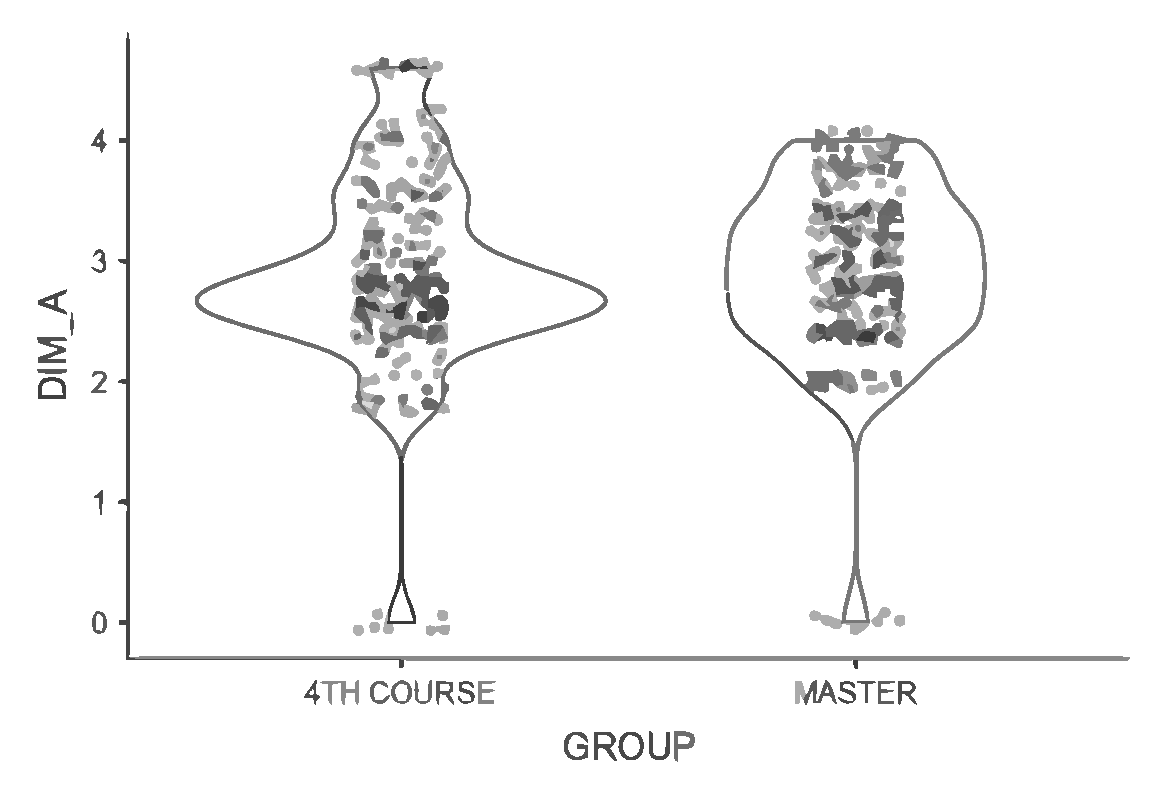
\includegraphics[width=0.5\textwidth]{fig1.png}
 \caption{\emph{Printscreen} da tela inicial do jogo Bruxa dos Acentos.}
 \label{fig1}
 \source{Bruxa dos Acentos.}
\end{figure}

Após o usuário apertar para iniciar o jogo, é apresentada a ele uma mensagem inicial que proporciona a primeira interação entre jogo-usuário, com a utilização do vocativo “pequeno aventureiro”, e também as primeiras instruções para o jogo: o jogador é convidado a enfrentar a Bruxa que rouba os acentos e a devolvê-los para que, enfim, ela seja derrubada da vassoura e não saia à caça novamente. É interessante observar que há mais recursos animados nessa parte, como morcegos voando e texto verbal que se move.

Ao começar o jogo, o cenário muda: agora, aparece um caldeirão de onde sai a palavra sem acento. Os acentos (agudo, circunflexo e grave) aparecem como possibilidades de ingredientes para a realização da poção da bruxa, conforme se vislumbra na \Cref{fig2}.

\begin{figure}[htbp]
 \centering
 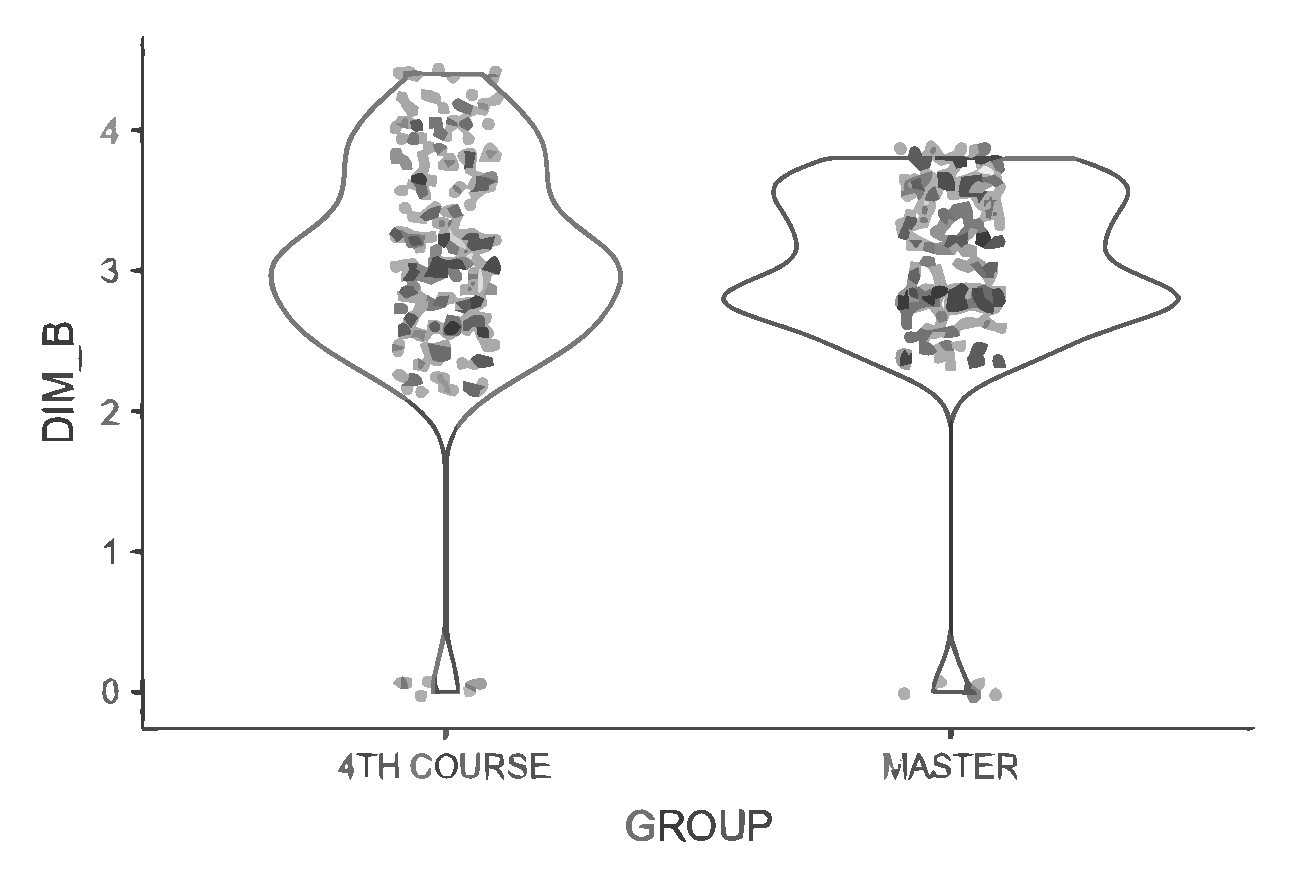
\includegraphics[width=0.5\textwidth]{fig2.png}
 \caption{\emph{Printscreen} da tela do jogo Bruxa dos Acentos.}
 \label{fig2}
 \source{Bruxa dos Acentos.}
\end{figure}

Logo, o jogador deve escolher um dos acentos e arrastá-lo até sua posição correta na palavra, para que possa seguir adiante. A cada acerto, a palavra muda; a cada erro, são dadas ao usuário três outras oportunidades de acerto. Caso ele erre pela quarta vez, a grafia correta lhe é oferecida, sem a justificativa. Após o quinto item aparecer, uma caveira surge no cenário. Se o participante não optar por apertá-la, novas palavras surgem; e, se clicar nela, ele não terá mais acesso às palavras, pois ele mudará de fase. Para esse segundo e último desafio, o objetivo é matar as bruxas, destruir as teias e os dragões que aparecem. Para atingi-lo, é dada a ordem: usar o canhão mágico para impedir que a bruxa roube mais acentos e atentar-se às teias de aranha que têm o poder de paralisá-lo e também às teclas que deve utilizar para disparar (o espaço) e movimentar o canhão (setas). Não há mais nenhuma abordagem em relação à acentuação. Após completados 100 pontos (cada elemento atingido vale uma quantia de pontos), o usuário finaliza e ganha o jogo.

Descrito o game, analisam-se agora os critérios didático-pedagógicos. Os dois primeiros a serem investigados são a concepção de língua e o tipo de ensino. Sobre isso, nota-se que o jogo traz as palavras a serem acentuadas completamente fora de qualquer contexto e aleatoriamente, e o que importa é a memorização da acentuação  – este é, inclusive, um dos objetivos elencados pelo site. Dessa forma, não havendo uma contextualização do fenômeno, a acentuação é estudada por si só, fora do uso real da língua, o que não é o ideal, pois se esperava uma aprendizagem ativa e contextualizada, além do ensino produtivo \cite{ribeiro2009}. De forma oposta ao desejado, constata-se, portanto, a exploração da acentuação numa concepção estruturalista \cite{costa_val1996, couto2020} e o ensino prescritivo da gramática, podendo ser fatores que dificultem a aprendizagem do corpo discente. Chama a atenção, além disso, a incoerência entre essa forma aleatória escolhida e a colocação da opção de uso do acento grave. Sabe-se que este acento marca a crase, e este fenômeno necessita de um contexto sintático para ser pensado. Além disso, para a idade do público-alvo selecionado, também considera-se inconveniente colocar o grave como sugestão, uma vez que não faz parte do universo dos estudantes ainda  – esse objeto de conhecimento é aprendido apenas nas séries finais do Ensino Fundamental II.

Em relação ao critério 3, sobre a disposição do objetivo e do conteúdo, percebem-se alguns pontos interessantes de serem discutidos. Na primeira página do jogo, encontra-se a informação do nível pensado para os usuários  – Ensino Fundamental I  –, das séries  – 2º, 3º e 4º anos  –, da idade  – 07 a 10 anos  – e da categoria  – Língua Portuguesa. Essas informações são importantes de serem mencionadas para orientar o professor sobre a adequação do jogo ao público-alvo. Ademais, o site traz “Dicas para o educador”, em que é fornecida a informação de que o jogo é um aliado ao trabalho de acentuação gráfica, já que é um recurso didático para fixação do conteúdo. Logo em seguida, observam-se os objetivos pedagógicos muito bem esclarecidos: i) aprimorar a leitura e a escrita, ii) reconhecer a necessidade de acentuar as palavras abordadas, percebendo a relação direta com a oralidade, iii) memorizar a acentuação das palavras, iv) fixar a aprendizagem dos sinais de acentuação e as marcas sonoras que representam; v) utilizar corretamente a acentuação na escrita de palavras usuais. Como defende \textcite{ribeiro2013}, essas informações, quando muito bem explicitadas, favorecem uma boa orientação quanto à seleção da ferramenta para adequação ao uso a partir do trabalho feito em sala de aula. Nesse sentido, o docente, ao buscar por um jogo de acentuação, verá se os objetivos elencados no game dialogam com os dele a fim de gerar uma melhor prática de ensino-aprendizagem.

Em relação especificamente ao conteúdo, não há nenhuma referência à forma como o jogo foi pensado, por exemplo, em relação às regras de acentuação. Não se tem, por exemplo, respostas a estas perguntas: a ordem de aparição das palavras depende da classificação em oxítona, paroxítona ou proparoxítona? Depende do tipo de acento, agudo, circunflexo ou grave? Ou da quantidade de sílabas? Ou ainda da formação do som, fechado ou aberto? Não se sabe, pois as palavras aparecem aleatoriamente. Logo, é percebido um problema quanto a isso, uma vez que a falta de esquematização dificulta, de acordo com \textcite[p. 77]{ribeiro2013}, “a percepção e a compreensão do aprendiz”.

O critério 4, a respeito dos recursos e da interatividade, já foi um pouco abordado acima. Há sons e bastantes animações que são muito adequadas à temática do jogo e à idade idealizada para brincar e que foram muito bem planejadas para atrair os olhares das crianças. Há, portanto, os elementos que proporcionarão a ludicidade do jogo. Ainda sobre os recursos lúdicos, é curiosa a associação entre bruxa e acentuação gráfica engendrada, pois, no senso comum, a acentuação é colocada como algo difícil, assim como a bruxa, muitas vezes, está ligada a uma representação do mal. Nessa lógica, até que ponto o jogo não fomentaria uma visão pejorativa sobre o aspecto linguístico, já que, pela narrativa, a bruxa estaria roubando o acento das palavras para produzir feitiçarias e praticar o mal com o diacrítico?

Além disso, \textcite{ribeiro2013} coloca como necessidade a existência de recursos que possibilitem a interação: entre usuário-conteúdo, que não é explorada, mesmo porque não é esquematizado, como já se discutiu sobre o conteúdo; entre usuário-professor, talvez a falta de temporizador para responder e também a possibilidade de errar até 3 vezes pode possibilitar a intervenção docente; e entre usuário-máquina, a qual é percebida com as teclas que permitem ao usuário autonomia e controle das atividades  – aspectos positivos na visão de \textcite{ribeiro2013}.

O critério 5 foi mal avaliado para este jogo. \textcite{ribeiro2009} dizem ser fundamental a sensação de estar aprendendo e, por isso, sendo recompensado. Porém, o jogo não explora de maneira bem definida uma motivação para que o usuário permaneça nele, mesmo porque não há menção, no início, de que ele pode ter a possibilidade de, ao acertar 5 palavras, passar para a 2ª fase. Isso só é descoberto se o discente chegar à quinta palavra. Ademais, quando é alcançada a 2ª fase, não é explicado que o usuário deve chegar aos 100 pontos, nem o valor que cada objeto destruído tem. Assim, não há elementos, além dos recursos visuais, que motivem a continuidade no jogo.

Por fim, os critérios 6 e 7. Quanto ao \emph{Feedback}, o 6, ou seja, aquela resposta dada ao jogador sobre o seu desempenho, não existe. Errando ou acertando, o participante não recebe orientações ou estímulos para seguir adiante, ou para entender seus erros: por exemplo, não há a justificativa da acentuação de cada palavra. O mesmo ocorre com o sete, o sistema de ajuda. O site não oferece ferramentas que possibilitem ajuda ao usuário quando ele necessitar. Esses dois pontos configuram-se, assim, como dificultadores do processo de aprendizagem.

Passa-se, a seguir, para os três critérios ergonômicos. O primeiro, a usabilidade, atende a todas as ideias que as autoras colocam. O jogo é de fácil uso, tem regras (apesar de poucas), enredo (um ponto positivo para a ludicidade) e arquitetura simples de ser entendida e manuseada, como defende \textcite{ribeiro2013}, e é, pois, uma interface intuitiva e autoexplicativa \cite{ribeiro2009}. Um único ponto a ser criticado é o momento de aparição da caveira para possibilitar a mudança de fase. Quando ela aparece, não há nenhuma informação que direcione o jogador a clicar nela, que pode permanecer na acentuação das palavras até desistir pela monotonia, ou pode clicar e perder a chance de testar mais seus conhecimentos sobre acentuação, já que, ao passar de fase, o elemento linguístico é abandonado.

Por fim, os dois últimos critérios. O jogo tem um bom nível de acessibilidade: pode ser acessível em qualquer lugar em que haja internet e também por qualquer pessoa, até mesmo aquelas com necessidades especiais. Em relação ao seu funcionamento, tem um excelente funcionamento, não trava e possui boas respostas às interações.

\subsection{Jogo 2: Acentuando}
O segundo jogo em questão, intitulado Acentuando, foi criado pela Estácio de Sá e pode ser baixado gratuitamente na loja de aplicativo para \emph{smartphones}. É compreendido pelo produtor como um jogo-aplicativo divertido para que o usuário treine os conhecimentos em acentuação. Sem qualquer tipo de animação, tem um layout mais clássico, nas cores azul, amarelo e bege, além de uma música de fundo instrumental que pode ser silenciada caso seja do interesse do jogador.

Na tela inicial, há um menu no qual consta uma divisão dos três tipos de acento da língua portuguesa: agudo, circunflexo e grave; conforme se vê na \Cref{fig3}:

\begin{figure}[htbp]
 \centering
 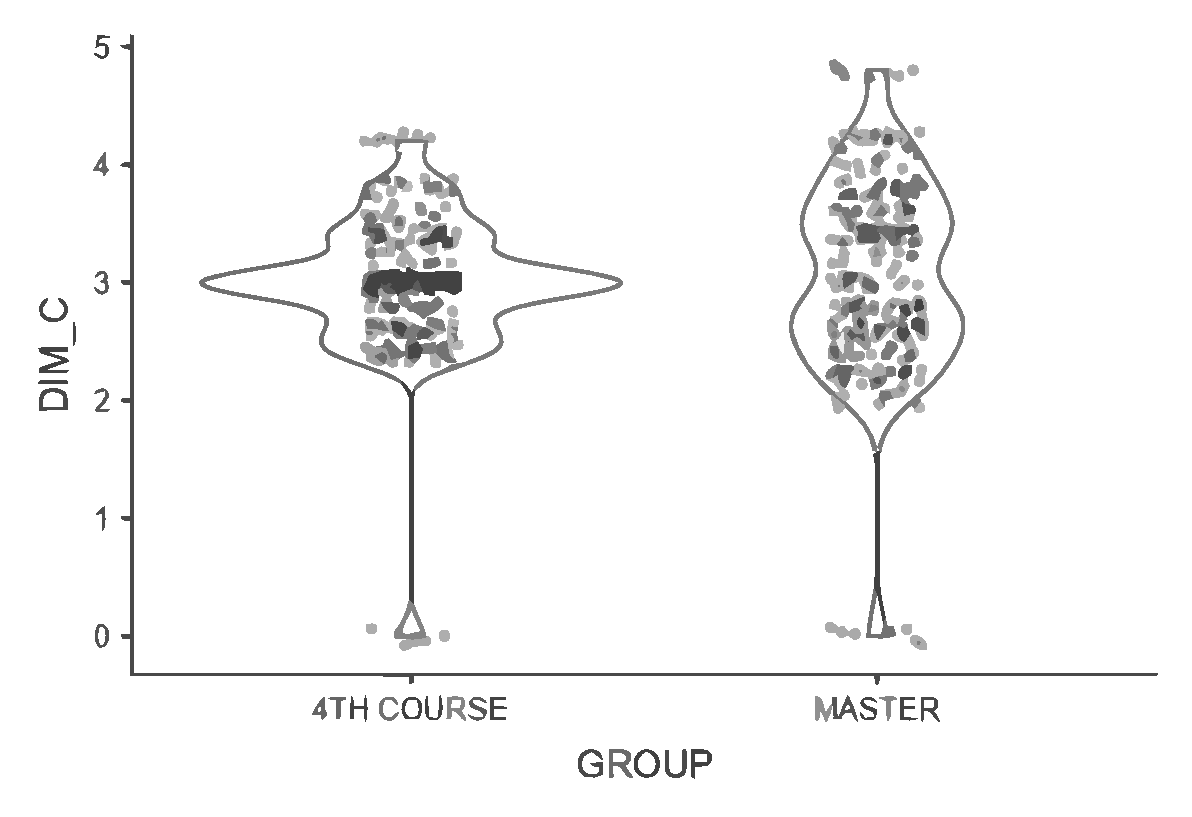
\includegraphics[width=0.5\textwidth]{fig3.png}
 \caption{\emph{Printscreen} da tela inicial do jogo Acentuando.}
 \label{fig3}
 \source{Acentuando.}
\end{figure}

Ao clicar em um desses três primeiros itens, aparecerão, a cada vez, dez perguntas objetivas – com duas alternativas (uma com, outra sem acento) – sobre cada tipo de acento, e o estudante deverá escolher a opção em que a palavra está grafada corretamente. Após optar por um vocábulo, surge uma mensagem de \emph{feedback} para indicar se a opção escolhida foi a certa ou não. Independentemente se o usuário erra ou acerta, junto dessa correção, sempre aparece uma regra que prescreve o acento (e que é exemplificada pelo par de palavras analisado) ou que proíbe o uso desse sinal gráfico, como se nota na \Cref{fig4}.

\begin{figure}[htbp]
 \centering
 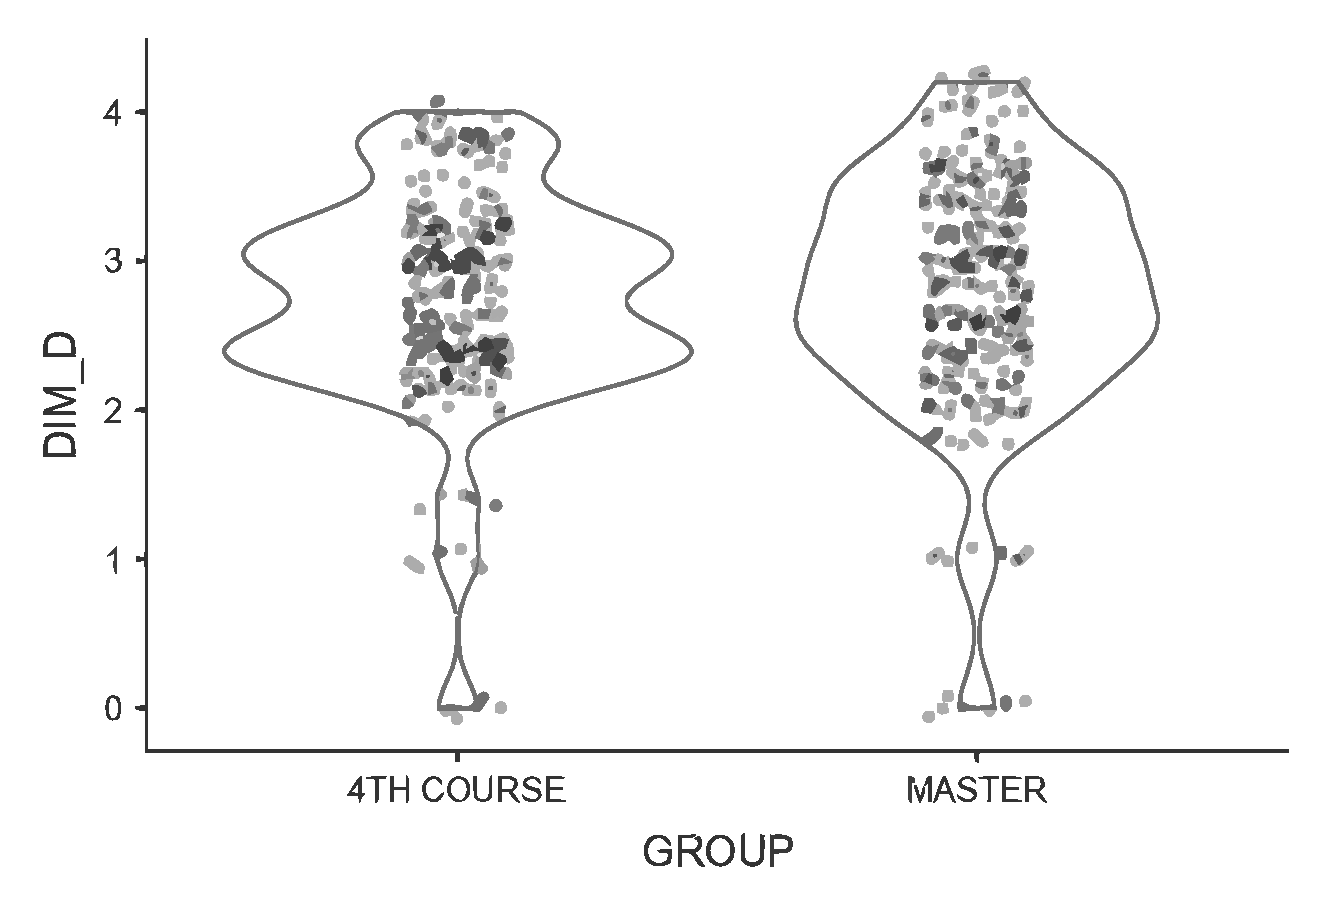
\includegraphics[width=0.5\textwidth]{fig4.png}
 \caption{\emph{Printscreen} do jogo Acentuando.}
 \label{fig4}
 \source{Acentuando.}
\end{figure}

Ao terminar as dez questões sobre um tipo de acento, o jogador recebe um percentual do seu desempenho até o momento no jogo, para cada item do menu (em números absolutos) e para seu desempenho geral (em porcentagem). Essa jogabilidade se mantém com a diferença de que, na parte do acento circunflexo e grave, a análise linguística não acontece apenas a partir de palavras isoladas, mas também de frases curtas em que há uma palavra que deve ou não estar acentuada. É interessante mencionar que essa opção por colocar frases curtas para acentos circunflexos se dá devido às palavras que recebem (ou não) acento diferencial, como “por”, ou aos critérios de concordância, no caso de “tem” (plural ou singular). No caso do grave, como já mencionado anteriormente, sabe-se que o conhecimento de sua colocação depende do contexto.

Finalizadas as dez perguntas para cada tipo de acento, o usuário é direcionado a um último desafio composto por dez questões de múltipla escolha, com cinco alternativas, transcritas de concursos públicos e que exigem noções sobre todos os acentos gráficos. Caso seja de interesse do jogador, ele pode refazer cada uma das quatro etapas (três específicas para cada tipo de acento e uma voltada a concursos) e outras palavras/frases são apresentadas para análise, isto é, o jogo conta com um banco de questões mais amplo (porém limitado) que as quarenta perguntas no total.

No que concerne aos dois primeiros critérios didático-pedagógicos, Concepção de língua e Tipo de ensino, pode-se dizer que, no jogo Acentuando, a língua é expressão do pensamento, reflexo da atividade mental \cite{costa_val1996, couto2020}, e, portanto, estudada de forma descontextualizada, por meio de palavras isoladas e/ou frases curtas, sem propósito sociocomunicativo; e o ensino, por sua vez, é do tipo prescritivo, sem reflexão, mas via exposição de regras (que não aparecem na Bruxa dos Acentos) a serem memorizadas e/ou relembradas pelos estudantes \cite{ribeiro2013, ribeiro2009}.

Quanto ao critério 3, Disposição do objetivo e do conteúdo, o jogo explicita que incentiva o estudo da acentuação de forma lúdica e não há qualquer indicação de público-alvo. Diferente do Bruxa dos Acentos, não aparecem também orientações para professores e/ou alunos nem são detalhados objetivos mais específicos; o que, para \textcite{ribeiro2013}, não é um ponto positivo. O conteúdo, entretanto, já é, em certo sentido, mais bem dividido, pois os exercícios com as regras são separados pelo tipo de acento, conforme se vislumbra na \Cref{fig2} já apresentada. Assim, o docente pode solicitar que os estudantes respondam às perguntas somente sobre acento circunflexo, por exemplo, o que, para \textcite{ribeiro2013}, facilita a escolha da ferramenta. Dentro de cada tipo de acento, todavia, não há uma gradação em níveis de dificuldade com relação ao conteúdo.

Sobre Recursos e Interatividade, critério 4, pode-se afirmar que o Acentuando apresenta três recursos multimodais – palavras, som e cores. Estes dois últimos são pouco explorados, uma vez que o som é único para todas as etapas do jogo (e pode, inclusive, ser silenciado) e as cores são constantes e pastéis. Não há contagem de tempo, animações ou quaisquer imagens, e facilmente a sequência de desafios poderia ser transposta para o papel, característica de jogos criticada por \textcite{ribeiro2009}. Em outras palavras, talvez até por não ter um público-alvo definido, o jogo não traz elementos lúdicos, nem fornece recursos que estabeleçam uma interação entre usuário e conteúdo e que propiciem uma aprendizagem prazerosa \cite{ribeiro2013}.

No critério 5, Motivação, embora o jogo apresente um percentual de desempenho do jogador, isso não gera neste engajamento, tendo em vista que não há uma valorização significativa para quem acerta, nem indicativos para se repensar sobre o erro. Ou seja, ao contrário do que postulam \textcite{ribeiro2009}, o jogo não favorece, de fato, a aprendizagem da escrita. Também não há uma progressão, em níveis de dificuldade, que estimule o usuário e que exija mais deste na medida em que se avança no jogo \cite{ribeiro2009}. Essas constatações têm estreita relação com o critério 6: \emph{Feedback}. Como já dito, havendo um erro ou um acerto, a regra de acentuação é explicitada, contudo isso não propicia reflexão nem a apreensão ativa das regras. Ademais, esse retorno avaliativo é o único Tipo de ajuda – aspecto compreendido no sétimo critério – para amparar o estudante. Logo, a análise empreendida permite a construção de uma avaliação negativa do jogo para os critérios 5, 6 e 7.

Por último, passa-se para a análise dos critérios ergonômicos. Em relação à Usabilidade, percebe-se que é um jogo muito fácil de ser usado, dispensando, assim, a apresentação de orientações muito específicas. Não há enredo elaborado, o que prejudica a questão da ludicidade, mas a arquitetura é de fácil entendimento também, sendo uma interface intuitiva e autoexplicativa \cite{ribeiro2009}. Os dois últimos critérios, Acessibilidade e Funcionamento, são bem avaliados para o jogo, uma vez que este pode ser acessado por todos que tenham um \emph{smartphone} com internet e por apresentar uma regularidade de atividade.

\section{Síntese das análises: em busca de aprendizagem e ludicidade}\label{sec-6}
A partir das análises feitas tendo como base os dez critérios elencados, compreende-se que os jogos digitais Bruxa dos Acentos e Acentuando, apesar de terem obtido um bom resultado nos critérios ergonômicos, afastam-se demasiadamente de conceituação de um bom jogo\footnote{Optou-se por continuar a denominar os objetos digitais analisados como jogos, apesar da aproximação com o conceito de “atividade interativa digital”, pois foi essa a nomeação dada pelos fabricantes.} proposta por \textcite{leffa2012}. Isso porque, em relação aos critérios didático-pedagógicos, promovem ludicidade, interatividade e imprevisibilidade mínimas ou nulas; tendo, assim, uma deficiência no quesito entretenimento. Na verdade,

\begin{quote}
muitas atividades mediadas por computador, às vezes descritas como games educativos pela sua interatividade, uso de áudio e animações, mas, com raras exceções, não passam de atividades tradicionais travestidas como jogo, na tentativa de ensinar e divertir ao mesmo tempo \cite[p. 224]{leffa2012}.
\end{quote}

Isso é exatamente o que se vislumbra nos jogos analisados, em especial no Acentuando, pois a mediação pedagógica é totalmente tradicional, porém realizada em um ambiente digital no qual é possível combinar diferentes linguagens, como cores, sons e palavras. \textcite{leffa2012}, inclusive, mencionam que esse tipo de atividade interativa em suporte eletrônico, em que são dados retornos automáticos aos jogadores, nem seria entendida como videogame por um amante do universo dos games, já que, sem diversão, o jogador não se sente motivado e – muito menos – vicia-se.

Embora um jogo sempre promova algum tipo de aprendizagem \cite{gee2004, jones2004, ribeiro2016}, é preciso reconhecer que, além de pouca, no caso do Bruxa dos Acentos, ou, no caso do Acentuando, da ausente ludicidade, os jogos  analisados também possibilitam uma tímida aprendizagem. Exemplos que corroboram isso são: a perspectiva tradicional – prescritiva, ora estruturalista, ora gerativista – de ensino-aprendizagem adotada nos jogos; o uso de palavras soltas e frases descontextualizadas; a falta de progressão do conteúdo e de recompensas ao jogador; a carência de \emph{feedback} ou a presença deste com exposição das regras a serem memorizadas passivamente; a ausência de reflexão na análise linguística etc. Essa análise vale tanto para o desenvolvimento de habilidades sobre a escrita, particularmente a acentuação gráfica, quanto para aquelas condizentes com a promoção do letramento digital, que também fica a desejar \cite{ribeiro2014}.

Diante desses resultados, em maioria, negativos em relação aos critérios didático-pedagógicos\footnote{Como o resultado dos critérios ergonômicos foi satisfatório, foram propostas diretrizes apenas para os critérios didático-pedagógicos.}, são propostas algumas diretrizes que devem ser levadas em conta na produção de um jogo focado na acentuação gráfica, de modo a haver uma conciliação entre ludicidade e aprendizagem \cite{leffa2012} (\Cref{tab1}).

\begin{table}[h!]
\caption{Proposições de melhorias nos jogos analisados}
\centering
\label{tab1}
\begin{tabular}{p{0.3\textwidth}p{0.3\textwidth}p{0.3\textwidth}}
\toprule
Critérios didático-pedagógicos & Bruxa dos Acentos & Acentuando
\\
%\arrayrulecolor[gray]{.7}
\midrule
Concepção de língua & \multicolumn{2}{p{0.6\textwidth+2\tabcolsep}}{Explorar, em vez de palavras soltas ou frases curtas, textos completos, preferencialmente de circulação real, para a análise da acentuação das palavras, seja para qualquer tipo de acento: agudo, circunflexo ou grave. Assim, tendo em vista que a gramática é inerentemente contextualizada \cite{antunes2014}, a aprendizagem seria mais construtiva e a concepção de língua seria interativa. Ademais, seria viável trabalhar com temas e, por consequência, com palavras – que devem ser acentuadas e que são frequentes – de um mesmo campo semântico.}
\\
\midrule
Tipo de ensino & \multicolumn{2}{p{0.6\textwidth+2\tabcolsep}}{No lugar de apenas apresentar as regras, ou o acerto ou o erro, permitir que o estudante entenda as relações linguísticas. Trazer, portanto, uma abordagem indutiva, em que ocorrerá a construção das regras pelo próprio aluno \cite{ludescher2006} em uma progressão de dificuldade.}
\\
\midrule
Disposição do objetivo e do conteúdo & Explicitar claramente a esquematização do conteúdo e a gradação de dificuldade. & Explicitar claramente as intenções pedagógicas.
\\
\midrule
Recursos e interatividade & Melhorar a forma de interação entre usuário-conteúdo, com regras bem definidas. & Adicionar recursos interativos/animados e melhorar todos os diálogos: usuário-máquina, usuário-conteúdo e usuário-professor. 
\\
\midrule
Motivação & \multicolumn{2}{p{0.6\textwidth+2\tabcolsep}}{Explorar elementos que motivem o usuário a continuar no jogo, como recompensas e desafios, sempre relacionados ao aprendizado da língua e a diferentes graus de dificuldade.}
\\
\midrule
\emph{Feeback} & \multicolumn{2}{p{0.6\textwidth+2\tabcolsep}}{Trazer um retorno às ações do usuário ricas o suficiente para fazer o jogador (re)pensar sobre seus erros e acertos. Nesse sentido, ao invés de explicitar a regra ou simplesmente omiti-la, seria interessante, por exemplo, aparecerem perguntas que façam o aprendiz refletir até ser capaz de construir hipóteses e generalizações.}
\\
\midrule
Sistemas de Ajuda & \multicolumn{2}{p{0.6\textwidth+2\tabcolsep}}{Inserir um hiperlink de ajuda automática, ou um recurso que possibilite a comunicação com o professor.}
\\
%\arrayrulecolor{black}
\bottomrule
\end{tabular}
\source{Autoria própria.}
\end{table}

\section{Considerações finais}\label{sec-7}
Este estudo teve como objetivo analisar como jogos digitais gratuitos podem (ou não) contribuir com o ensino e a aprendizagem da acentuação gráfica. Para alcançar esse propósito, foram analisados dois jogos, Bruxa dos Acentos e Acentuando. Lamentavelmente, os dois jogos, assim denominados por seus criadores, distanciam-se demasiadamente da conceituação de um bom jogo proposto por \textcite{leffa2012}, pois a ludicidade, a interatividade e a imprevisibilidade não foram devidamente exploradas. Concorda-se com \textcite{leffa2012} de que os games deveriam ser compreendidos como uma prática social que pode favorecer oportunidades de uso da língua, em contextos reais ou simulados. Além disso, é indispensável haver estreita ligação entre aprendizagem e ludicidade, para que o aluno deseje jogar o game e, por meio dele, aprenda sobre a língua \cite{leffa2012}. 

Nessa direção, os jogos Bruxa dos Acentos e o Acentuando deveriam ser vistos, em sintonia às teorias adotadas, como atividades interativas digitais \cite{leffa2012}. Em outras palavras, as conexões entre ludicidade e aprendizagem dos dois recursos didáticos analisados não foram totalmente possíveis, porque, na verdade, ainda estão muito ligados a uma lógica tradicional, mecânica e descontextualizada de se ensinar a acentuação gráfica e, consequentemente, de se aprender tal conteúdo. Para que tais objetos digitais possam ser considerados jogos digitais pedagógicos, melhorias são necessárias, como utilizar uma concepção de língua sociointeracionista, que busque levar os alunos à reflexão sobre a língua e as relações linguísticas que envolvam a acentuação gráfica, por meio de um contexto; além de haver interatividade e ludicidade, que possam despertar nos discentes o interesse em aprender a respeito dos fenômenos da língua por meio da qual interagem. Dessa forma, os jogos poderão contribuir com o ensino da língua escrita e, por conseguinte, com o desenvolvimento do aluno letrado, que seja capaz de utilizar as diversas facetas da língua, como a relativa à escrita ortográfica – especificamente a acentuação gráfica – nos mais diversos contextos sociais em que esse conhecimento é exigido \cite{soares2004, soares2018}. 

Futuras pesquisas sobre o tema deste artigo poderão ser desenvolvidas, com objetivos tais como: analisar a percepção de uso dos estudantes em relação ao Bruxa dos Acentos e ao Acentuando; desenvolver um jogo digital que ofereça ao discente a possibilidade de refletir com ludicidade sobre os aspectos relacionados à acentuação gráfica; investigar o impacto de jogos digitais no desempenho linguístico do alunado nas aulas de Língua Portuguesa. Outras investigações ainda poderão se debruçar sobre outros jogos digitais que abarcam diferentes conteúdos pertencentes ao escopo do componente curricular LP, tendo em vista que essa associação é imprescindível à educação na atualidade. Por fim, espera-se que as discussões sobre os jogos digitais no ensino da Língua Portuguesa não cessem, e este trabalho possa ser porta-voz de novas discussões e pesquisas nessa área.

\printbibliography\label{sec-bib}
% if the text is not in Portuguese, it might be necessary to use the code below instead to print the correct ABNT abbreviations [s.n.], [s.l.] 
%\begin{portuguese}
%\printbibliography[title={Bibliography}]
%\end{portuguese}

%full list: conceptualization,datacuration,formalanalysis,funding,investigation,methodology,projadm,resources,software,supervision,validation,visualization,writing,review
\begin{contributors}[sec-contributors]
\authorcontribution{Ana Luiza de Souza Couto}[review,visualization]
\authorcontribution{Letícia Pena Silveira}[datacuration,investigation,methodology]
\authorcontribution{Marcelo de Castro}[conceptualization,writing]
\end{contributors}


\end{document}
